
\section{Ablation Studies} \label{app:ablation}

Here we conduct ablation studies to see 1) the influence of  using different quantiles to perform clipping; 2) the influence of varying the privacy budget for quantile estimation; 3) whether adaptive flat clipping significantly better than fixed flat clipping.


\paragraph{Clipping with Different Target Quantiles.}
We use different target quantiles for clipping on both WRN16-4 and RoBERTa-base. We choose the quantile for CIFAR-10 from $\{0.3,0.4,0.5,0.6,0.7,0.8,0.9\}$ and that for SST-2 from $\{0.05, 0.2, 0.4, 0.6, 0.85, 0.9, 0.95\}$. Other hyperparameters  are the same as those in Section~\ref{subsec:cifar10} and~\ref{subsec:roberta}. We plot the results in Figure \ref{fig:ablation-1-target-quantile}. On CIFAR-10, the accuracy is robust to the choice of target quantile on all values considered. On SST-2, all quantiles around $0.9$ give good performance. This suggests that setting the target quantile according to the model accuracy is a good default choice for the classification tasks. For generation task, we tune the target quantile as a hyper-parameter in general.

\begin{figure}
\centering
\begin{subfigure}[!t]{0.5\textwidth}
    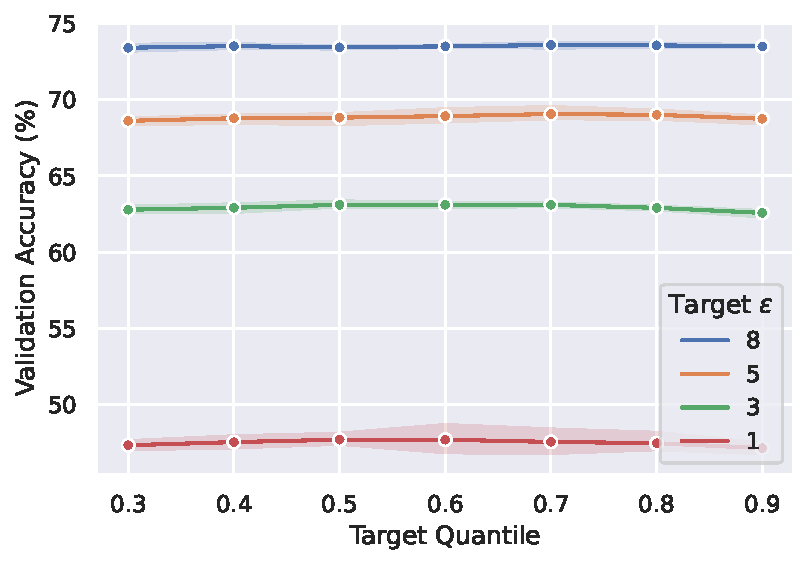
\includegraphics[width=\textwidth]{files/fig/ablation_1_cifar_rescale.pdf}
    \caption{CIFAR-10}
    \label{fig:ablation_1_cifar}
\end{subfigure}\hfill
\begin{subfigure}[!t]{0.5\textwidth}
    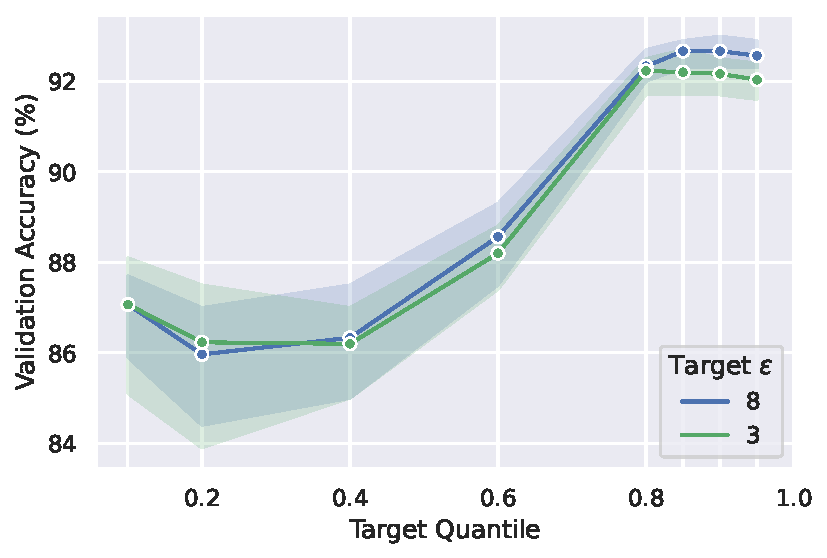
\includegraphics[width=\textwidth]{files/fig/ablation_1_sst.pdf}
    \caption{SST-2}
    \label{fig:ablation_1_sst2}
\end{subfigure}\hfill

\caption{Validation accuracy (in \%) with different target quantiles.
}
  \label{fig:ablation-1-target-quantile}
\end{figure}

\paragraph{Different Budgets for Quantile Estimation.}
We show the influence of using different privacy budgets to estimate the target quantile. We fine-tune RoBERTa-base models on SST-2. The fraction of privacy budget for quantile estimation $r$ is from $\{0.01\%, 0.1\%, 1\%, 5\%, 10\%, 20\%, 40\%, 80\%\}$. We plots the results in Figure \ref{fig:ablation-2-quantile-budget}. The performance is good for a wide range  of $r$. When $\epsilon=8$, using $r$ as small as $0.01\%$ still gives good accuracy. This further confirms the finding in \cite{andrew2019differentially} that quantiles can be estimated quite accurately with small privacy budget. Therefore we only need to split negligible budget for the private quantile estimation without affecting much the noises added to the model updates.

\begin{figure}[!t]
\centering
  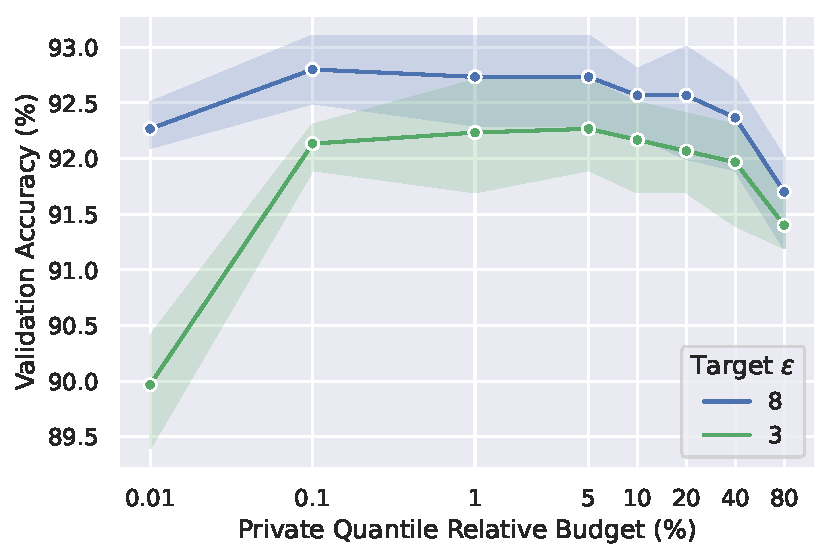
\includegraphics[width=0.5\linewidth]{files/fig/ablation_2.pdf}
  \caption{Validation accuracy (in \%) on SST-2 of using different budgets for quantile estimation.}
  \label{fig:ablation-2-quantile-budget}
\end{figure}
 
\paragraph{Adaptive Per-layer Clipping vs Adaptive Flat Clipping.} 
We have verified that adaptive per-layer clipping can match the performance of well-tuned flat clipping in Section~\ref{sec:experiment}. To really justify value of adaptive per-layer clipping, we need to demonstrate that adaptive flat clipping does not achieve significantly better performance than fixed flat clipping. We run experiments on the CIFAR-10 task with WRN16-4 and the SST-2 task with RoBERTa-base model. Their results are presented in Table~\ref{table:ablation_4_fixed_perlayer_cifar10} and Table~\ref{table:ablation_4_fixed_perlayer_sst2}. We can see that adaptivity also helps flat clipping but the improvement is not statistically significant. The performance of adaptive per-layer clipping is on par with that of adaptive flat clipping as well.
\begin{table}[h]
\footnotesize
\setlength\tabcolsep{2.4pt}
\caption{Adaptivity helps flat clipping but not as much as for per-layer clipping. Averaged accuracy and standard deviation are given by 3 independent runs.}

\newcommand{\bb}[1]{\textbf{#1}}

\begin{subtable}[h]{0.45\textwidth}
\centering
\caption{CIFAR-10}
\begin{tabular}{l ccc ccc}
\toprule
{Method} & 
\text{$\epsilon=3$} & 
\text{$\epsilon=8$} \\
\midrule
\textbf{Flat clipping} \\
\hspace{4mm} fixed & $63.1_{(0.22)}$ & $73.9_{(0.87)}$ \\ 
\hspace{4mm} adaptive & - & - \\[1.5mm] %
 & \bb{+$0$} & \bb{+$0$} \\ 
\midrule
\textbf{Per-layer clipping} \\
\hspace{4mm} fixed & $60.6_{(0.79)}$ & $67.8_{(1.20)}$ \\ %
\hspace{4mm} adaptive & $63.7_{(0.34)}$ & $73.5_{(0.87)}$ \\[1.5mm] %
  & \bb{+$3.1$} & \bb{+$5.7$} \\
\bottomrule
\end{tabular}
\label{table:ablation_4_fixed_perlayer_cifar10}
\end{subtable}
\hfill
\begin{subtable}[h]{0.45\textwidth}
\centering
\caption{SST-2}
\begin{tabular}{l ccc ccc}
\toprule
{Method} & 
\text{$\epsilon=3$} & 
\text{$\epsilon=8$} \\
\midrule
\textbf{Flat clipping} \\
\hspace{4mm} fixed & $91.5_{(1.07)}$ & $92.0_{(0.67)}$ \\ %
\hspace{4mm} adaptive & $92.2_{(0.70)}$ & $92.6_{(0.46)}$ \\[1.5mm] %
  & \bb{+$0.7$} & \bb{+$0.6$} \\ 
\midrule
\textbf{Per-layer clipping} \\
\hspace{4mm} fixed & $89.4_{(1.04)}$ & $89.7_{(0.70)}$ \\ 
\hspace{4mm} adaptive & $92.0_{(0.23)}$ & $92.4_{(0.44)}$ \\[1.5mm] %
  & \bb{+$2.6$} & \bb{+$2.7$} \\ 
\bottomrule
\end{tabular}
\label{table:ablation_4_fixed_perlayer_sst2}
\end{subtable}

\label{table:ablation_4_fixed_perlayer}
\end{table}










